% begin module optimization-ex5
\begin{frame}
\begin{example} %[Example 5, p. 303]
Find the largest possible area of a rectangle inscribed in a semicircle of radius $r$.
\begin{columns}[c]
\column{.5\textwidth}
\psset{xunit=1.8cm, yunit=1.8cm}
\begin{pspicture}(-1.5,-0.5)(1.6,1.4)
\psframe*[linecolor=white](-1.5,-0.5)(1.6,1.4)
\tiny
\psaxes[ticks=none, labels=none]{<->}(0,0)(-1.5,-0.5)(1.5,1.3)
%Function formula: sqrt{}(1- ((x)^{2}))
\psplot[linecolor=black, plotpoints=1000]{-1}{1}{x 2 exp -1 mul 1 add sqrt }
\rput[t](1,-0.1){$r$}
\rput[t](-1,-0.1){$-r$}

\uncover<10->{
\psline[linecolor=red](-0.866025404, 0.5,)(0.866025404, 0.5)
\psline[linecolor=red](-0.866025404, 0)(-0.866025404, 0.5)(0.866025404, 0.5)(0.866025404, 0)
\psline{<-}(-0.866025404, 0.4)(0.1, 0.4)
\rput(0.25, 0.4){$2x$}
\psline{->}(0.4,0.4) (0.866025404, 0.4)
\fcFullDot{0.866025404}{0.5}
\rput[bl](0.866025404,0.6){$(x,y)$}
}
\uncover<2>{
\psline[linecolor=red](-0.9, 0) (-0.9, 0.43589) (0.9, 0.43589) (0.9, 0)
}
\uncover<3>{
\psline[linecolor=red](-0.8, 0) (-0.8, 0.6) (0.8, 0.6) (0.8, 0)
}
\uncover<4>{
\psline[linecolor=red](-0.7, 0) (-0.7, 0.714143) (0.7, 0.714143) (0.7, 0)
}
\uncover<5>{
\psline[linecolor=red](-0.6, 0) (-0.6, 0.8) (0.6, 0.8) (0.6, 0)
}
\uncover<6>{
\psline[linecolor=red](-0.5, 0) (-0.5, 0.866025) (0.5, 0.866025) (0.5, 0)
}
\uncover<7>{
\psline[linecolor=red](-0.4, 0) (-0.4, 0.916515) (0.4, 0.916515) (0.4, 0)
}
\uncover<8>{
\psline[linecolor=red](-0.3, 0) (-0.3, 0.953939) (0.3, 0.953939) (0.3, 0)
}
\uncover<9>{
\psline[linecolor=red](-0.2, 0) (-0.2, 0.979796) (0.2, 0.979796) (0.2, 0)
}
\end{pspicture}
%\ \only<handout:0| -2>{%
%\uncover<2>{%
%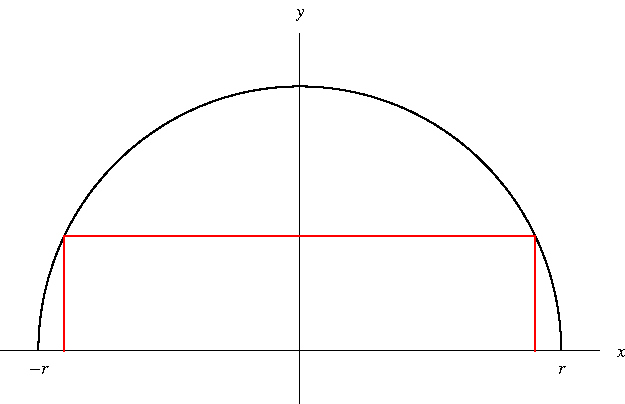
\includegraphics[width=5cm]{optimization/pictures/04-07-ex5a.pdf}%
%}}%
%\only<handout:0| 3>{%
%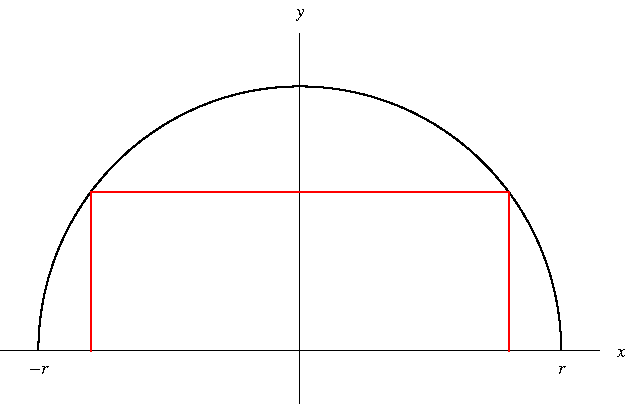
\includegraphics[width=5cm]{optimization/pictures/04-07-ex5b.pdf}%
%}%
%\only<handout:0| 4>{%
%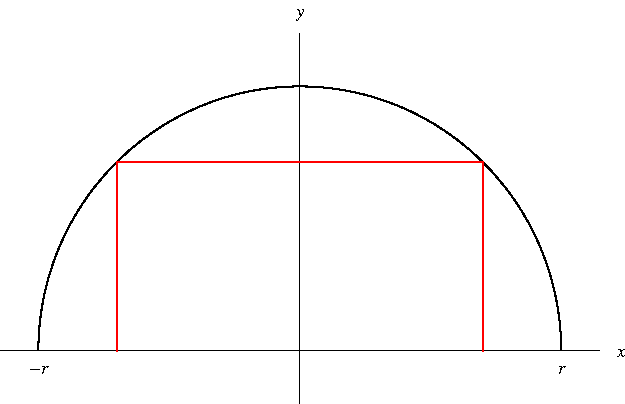
\includegraphics[width=5cm]{optimization/pictures/04-07-ex5c.pdf}%
%}%
%\only<handout:0| 5>{%
%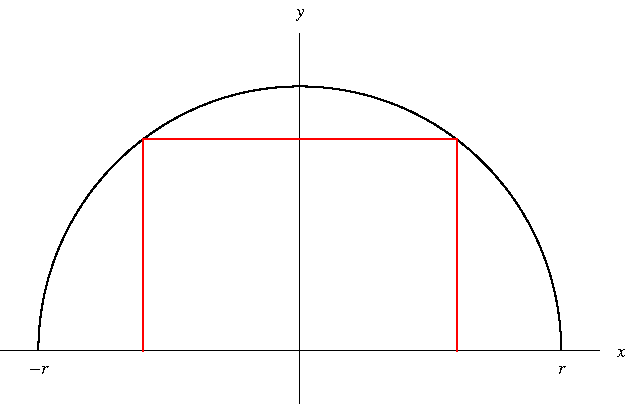
\includegraphics[width=5cm]{optimization/pictures/04-07-ex5d.pdf}%
%}%
%\only<handout:0| 6>{%
%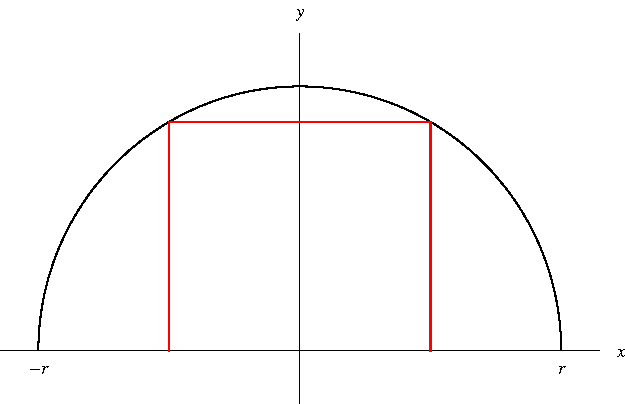
\includegraphics[width=5cm]{optimization/pictures/04-07-ex5e.pdf}%
%}%
%\only<handout:0| 7>{%
%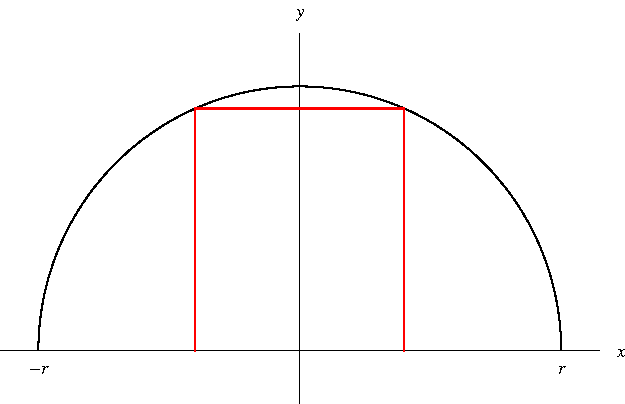
\includegraphics[width=5cm]{optimization/pictures/04-07-ex5f.pdf}%
%}%
%\only<handout:0| 8>{%
%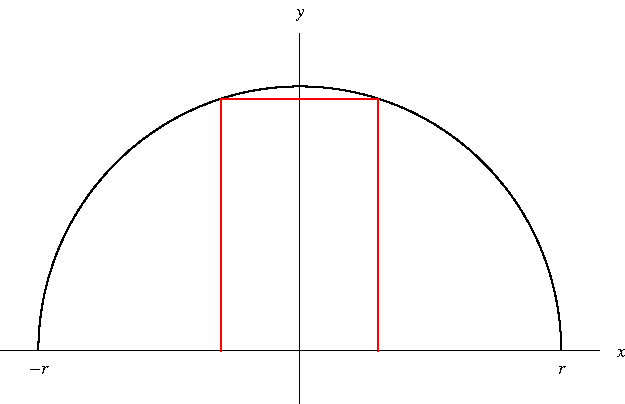
\includegraphics[width=5cm]{optimization/pictures/04-07-ex5g.pdf}%
%}%
%\only<handout:0| 9>{%
%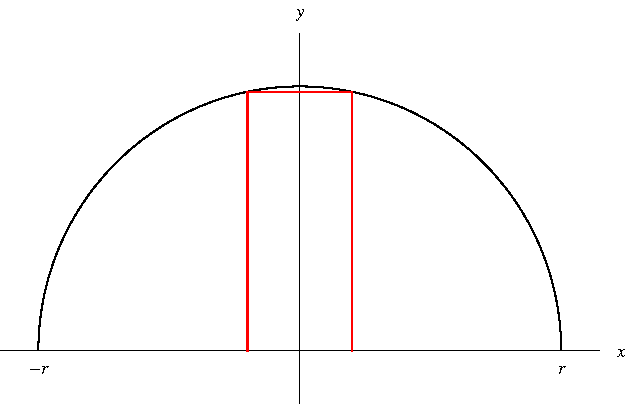
\includegraphics[width=5cm]{optimization/pictures/04-07-ex5h.pdf}%
%}%
%\only<10->{%
%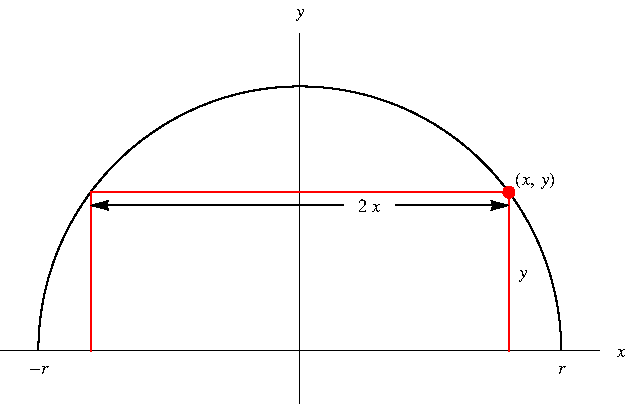
\includegraphics[width=5cm]{optimization/pictures/04-07-ex5i.pdf}%
%}%
\uncover<12->{To eliminate $y$, use the fact that $(x,y)$ lies on the semicircle.}%
\abovedisplayskip=0pt
\belowdisplayskip=0pt
\abovedisplayshortskip=0pt
\belowdisplayshortskip=0pt
\begin{align*}
\uncover<12->{y^2} & \uncover<12->{=}  \uncover<12->{r^2-x^2}\\
\uncover<13->{\alert<handout:0| 15>{y}} & \uncover<13->{\alert<handout:0| 15>{=}}  \uncover<13->{\alert<handout:0| 15>{\sqrt{r^2-x^2}}}%
\end{align*}
%\uncover<20->{%
%\abovedisplayskip=0pt
%\belowdisplayskip=0pt
%\[
%\begin{array}{r|r}
%x & A(x)\\
%\hline
%\alert<handout:0| 21-22>{0} & \alert<handout:0| 22>{\uncover<22->{0}}\\
%\alert<handout:0| 23-24,27>{600} & \alert<handout:0| 24,27>{\uncover<24->{720,000}}\\
%\alert<handout:0| 25-26>{2400} & \uncover<26->{\alert<handout:0| 26>{0}}
%\end{array}
%\]
%}%
\column{.5\textwidth}
\uncover<10->{%
Let the semicircle have center at the origin.  Let $(x,y)$ be the coordinates of the top right corner of the rectangle.  Let $A$ be its area.
}%

\uncover<14->{Notice that $0\leq x \leq r$.}
\abovedisplayskip=0pt
\belowdisplayskip=0pt
\abovedisplayshortskip=0pt
\belowdisplayshortskip=0pt
\begin{align*}
\uncover<11->{A} & \uncover<11->{=}  \uncover<11->{2x\alert<handout:0| 15>{y}}  \uncover<15->{=}  \uncover<15->{2x\alert<handout:0| 15>{\sqrt{r^2-x^2}}}\\
\uncover<16->{\alert<handout:0| 16-17>{A'}} & \uncover<16->{\alert<handout:0| 16-17>{=}}  \uncover<17->{\alert<handout:0| 17>{2\sqrt{r^2-x^2} - \frac{2x^2}{\sqrt{r^2-x^2}}}}\\
& \uncover<18->{=}  \uncover<18->{\frac{2(r^2-2x^2)}{\sqrt{r^2-x^2}}}
\end{align*}

\uncover<19->{%
Critical number: \alert<handout:0| 19-20>{$x = $ \uncover<20->{$\frac{r}{\sqrt{2}}$.}}
}%
\end{columns}
\uncover<21->{%
There is a local max. here because $A(0) = 0 = A(r)$.  Therefore the maximum area is $A(\frac{r}{\sqrt{2}}) = $ $ 2\frac{r}{\sqrt{2}}\sqrt{r^2 - \frac{r^2}{2}} = r^2$, achieved for $x=y=\frac{r}{\sqrt{2}}$
}%
\end{example}
\end{frame}
% end module optimization-ex5
